\documentclass[12pt,a4paper]{article}
\usepackage[utf8]{inputenc}
\usepackage[T1]{fontenc}
\usepackage[brazil]{babel}
\usepackage{geometry}
\usepackage{graphicx}
\usepackage{float}
\usepackage{booktabs}
\usepackage{listings}
\usepackage{xcolor}
\usepackage{hyperref}
\geometry{margin=2.5cm}

\lstdefinelanguage{VHDL}{
  morekeywords={library,use,entity,is,port,in,out,inout,architecture,of,begin,end,signal,process,if,then,else,elsif,case,when,others,downto,to,constant,variable,function,return,wait,until,rising_edge,falling_edge,generic,map,type,not,and,or},
  sensitive=true,
  morecomment=[l]--,
  morestring=[b]"
}

\lstset{
  language=VHDL,
  basicstyle=\ttfamily\small,
  keywordstyle=\color{blue!70!black},
  commentstyle=\color{green!40!black},
  numbers=left,
  numberstyle=\tiny,
  breaklines=true,
  frame=single,
  showstringspaces=false
}

\title{MC613 -- Relatório 3\\Projeto: Controlador DRAM}
\author{Rodrigo Banin Ferraz de Camargo (238257)}
\date{Junho de 2026}

\begin{document}
\maketitle
\tableofcontents
\newpage

\section{Planejamento}
O planejamento foi orientado pelos requisitos da entrega final: implementar um
controlador SDRAM funcional, integrá-lo com a interface da placa DE1-SoC e validar
por simulação os fluxos obrigatórios (INIT, READ, WRITE, REFRESH e WRITE seguido de
READ automático).

A arquitetura foi dividida em camadas para reduzir a complexidade e permitir a
validação incremental de cada parte:
\begin{itemize}
  \item \texttt{dram\_iface}: camada de interação com o usuário (SW/KEY/HEX), que
        traduz ações em requisições de leitura/escrita por meio do handshake
        \texttt{req}/\texttt{ready}.
  \item \texttt{reader}: pequeno registrador (buffer) que segura uma requisição
        estável entre a interface e a FSM de protocolo até o controlador consumi-la.
  \item \texttt{dram\_controller}: camada de protocolo SDRAM, responsável pelos
        comandos (ACTIVATE, READ, WRITE, PRECHARGE, AUTO REFRESH, LOAD MODE) e por
        toda a temporização crítica.
  \item \texttt{dram\_top\_level}: integração com a PLL, com a interface de usuário
        e com os pinos físicos da SDRAM.
\end{itemize}

Essa separação permitiu uma evolução incremental: primeiro validar a emissão de
requisições da interface, depois validar a temporização do controlador, e por fim
validar a integração completa entre os dois.

\subsection{Diagramas da etapa inicial}
\begin{figure}[H]
  \centering
  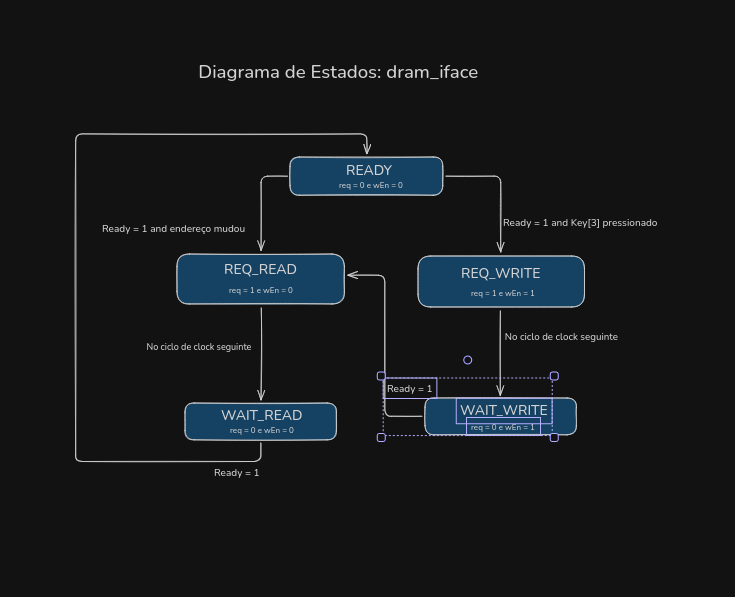
\includegraphics[width=0.95\textwidth]{dram_iface.png}
  \caption{Diagrama de estados do módulo \texttt{dram\_iface}.}
\end{figure}

\begin{figure}[H]
  \centering
  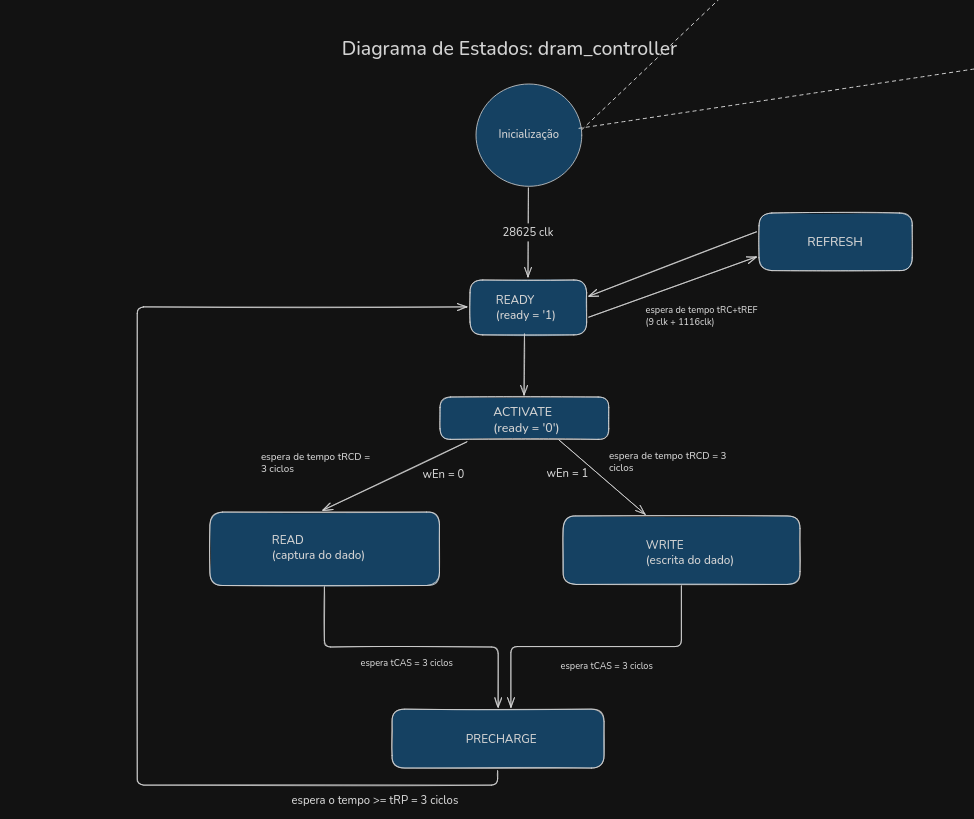
\includegraphics[width=0.95\textwidth]{controller.png}
  \caption{Diagrama de estados do módulo \texttt{dram\_controller}.}
\end{figure}

\begin{figure}[H]
  \centering
  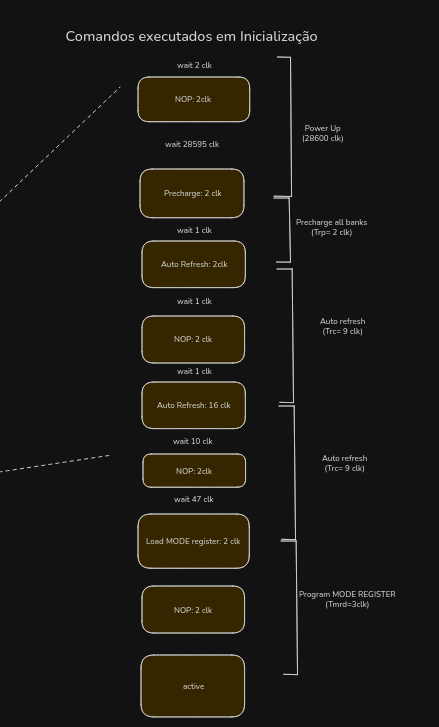
\includegraphics[width=0.95\textwidth]{init_commands.png}
  \caption{Sequência de inicialização da SDRAM (PRECHARGE ALL, 8 AUTO REFRESH,
  LOAD MODE REGISTER).}
\end{figure}

\section{Estrutura do Código}
\subsection{Arquivos sintetizáveis}
\begin{itemize}
  \item \texttt{dram\_iface.vhd}
  \item \texttt{reader.vhd}
  \item \texttt{dram\_controller.vhd}
  \item \texttt{dram\_top\_level.vhd}
  \item \texttt{pll.vhd} / \texttt{pll.qip} (megafunção de PLL da Altera, gera o
        clock interno a partir de \texttt{CLOCK\_50}).
\end{itemize}

\subsection{Arquivos de simulação}
\begin{itemize}
  \item \texttt{pll\_sim\_stub.vhd}: substituto da PLL \textbf{apenas em simulação}
        (o ghdl não elabora a megafunção Altera). Mantém a mesma entidade
        \texttt{pll} e gera um clock de aproximadamente 143~MHz, levantando
        \texttt{locked} após alguns ciclos. Nunca é sintetizado.
  \item \texttt{tb\_dram\_iface.vhd}: valida isoladamente a FSM de interface.
  \item \texttt{tb\_dram\_controller.vhd}: valida isoladamente o protocolo e a
        temporização do controlador.
  \item \texttt{tb\_dram\_top\_level.vhd}: valida a integração ponta a ponta do
        sistema completo.
\end{itemize}

\subsection{Descrição dos componentes}
\textbf{\texttt{dram\_iface}:} gera \texttt{req}/\texttt{wEn}, detecta escrita por
borda de descida de \texttt{KEY[3]}, dispara leitura ao detectar mudança de
endereço e faz leitura automática após cada escrita. Também sincroniza
\texttt{SW}/\texttt{KEY} com dois flip-flops (anti-metaestabilidade) e dirige os
displays de 7 segmentos (\texttt{HEX0}, \texttt{HEX1}, \texttt{HEX4}, \texttt{HEX5}).

\textbf{\texttt{reader}:} captura uma requisição de comando, mantém
endereço/dado/modo de escrita estáveis e só libera a FSM principal quando o
controlador confirma o consumo por \texttt{cmd\_ack}.

\textbf{\texttt{dram\_controller}:} consome os comandos bufferizados pelo
\texttt{reader} e executa o protocolo SDRAM (inicialização, ACTIVATE, READ, WRITE,
PRECHARGE, AUTO REFRESH e LOAD MODE), aplicando todas as esperas de temporização e
capturando o dado de leitura do barramento \texttt{DRAM\_DQ}. A espera de power-up
foi parametrizada por um \emph{generic} \texttt{INIT\_WAIT\_CYCLES} (padrão 28600).

\textbf{\texttt{dram\_top\_level}:} integra a PLL, a interface de usuário e os pinos
físicos da SDRAM, roteando o vetor de comando de 26 bits do controlador para os
pinos \texttt{DRAM\_*} e tratando o barramento bidirecional \texttt{DRAM\_DQ}.

\section{Implementação}
\subsection{Decisões centrais de implementação}
\begin{itemize}
  \item FSM com estados intermediários de espera dedicados para cada tempo crítico
        (tRCD, tRP, CAS latency, tRFC, tMRD);
  \item uso do \texttt{reader} como registrador de comando entre a interface e a
        FSM de SDRAM, com handshake por \texttt{cmd\_ack};
  \item codificação explícita dos comandos SDRAM por constantes de 26 bits
        (comando + endereço no mesmo vetor \texttt{adress});
  \item \textbf{captura do dado de leitura na borda de descida do clock} --- a
        correção mais importante do projeto (Seção~\ref{sec:analise});
  \item parametrização da espera de inicialização por \emph{generic}, para acelerar
        a simulação sem alterar o comportamento sintetizado;
  \item controle explícito da direção do barramento \texttt{DRAM\_DQ}: o top-level
        só o dirige no ciclo exato do comando WRITE.
\end{itemize}

\subsection{Trechos essenciais de código}

\subsubsection{Buffer de comando no \texttt{reader}}
\begin{lstlisting}[caption={Captura do comando ate o acknowledge do controlador (reader.vhd).}]
-- Se o controlador reconhece o comando, limpa o pendente
if cmd_ack = '1' then
  pending_reg <= '0';
end if;

-- Captura nova requisicao (inclusive no mesmo ciclo do ack, p/ fluxo continuo)
if req_in = '1' and (pending_reg = '0' or cmd_ack = '1') then
  pending_reg <= '1';
  wEn_reg     <= wEn_in;
  addr_reg    <= addr_in;
  data_reg    <= data_in;
end if;
\end{lstlisting}

\subsubsection{Arbitragem no estado READY do controlador}
\begin{lstlisting}[caption={Refresh tem prioridade sobre uma nova requisicao externa (dram\_controller.vhd).}]
when st_ready =>
  ready <= '1';
  if refresh_due = '1' then
    ready        <= '0';
    adress       <= CMD_PREALL;
    timer_cycles <= TRP_WAIT_CYCLES; timer_start <= '1';
    op_state     <= st_refresh_trp;
  elsif buffered_req = '1' then
    ready        <= '0';
    cmd_ack      <= '1';
    active_addr  <= buffered_addr;
    active_wen   <= buffered_wen;
    active_data  <= buffered_data;
    adress       <= command_with_address(CMD_ACTIVATE, buffered_addr,
                                          row_address(buffered_addr));
    timer_cycles <= TRCD_WAIT_CYCLES; timer_start <= '1';
    op_state     <= st_activate_wait;
  end if;
\end{lstlisting}

\subsubsection{Captura de leitura na borda de descida}
\begin{lstlisting}[caption={A janela valida do dado cai entre as bordas de subida; capturar na descida acerta (dram\_controller.vhd).}]
-- DRAM_CLK = not pll_clk, entao a borda de descida de clk coincide com a
-- borda de subida do clock do chip. A 143 MHz, o dado valido (tAC apos a
-- borda) cai ENTRE as subidas do sistema; capturar na descida le o valor
-- correto em vez de amostrar o barramento ainda em alta impedancia (0xFF).
dq_capture : process(clk, rst)
begin
  if rst = '1' then
    dq_in_reg <= (others => '0');
  elsif falling_edge(clk) then
    dq_in_reg <= data_in;
  end if;
end process;
\end{lstlisting}

\subsubsection{Leitura automática pós-escrita no \texttt{dram\_iface}}
\begin{lstlisting}[caption={Ao fim da escrita, a propria interface dispara um READ de confirmacao (dram\_iface.vhd).}]
when WAIT_WRITE_ST =>
  if ready = '1' then
    req_reg <= '1';   -- dispara leitura de confirmacao
    wen_reg <= '0';
    state   <= REQ_READ_ST;
  end if;
\end{lstlisting}

\subsubsection{Direção do barramento e integração no top-level}
\begin{lstlisting}[caption={O top-level so dirige DRAM\_DQ no comando WRITE e instancia o controlador (dram\_top\_level.vhd).}]
-- So dirige DRAM_DQ durante o WRITE (CS=0, RAS=1, CAS=0, WE=0); senao alta-Z
DRAM_DQ <= (x"00" & controller_write_data)
           when (dram_cmd(18)='0' and dram_cmd(17)='1' and
                 dram_cmd(16)='0' and dram_cmd(15)='0')
           else (others => 'Z');

controller_i : dram_controller
  generic map (INIT_WAIT_CYCLES => INIT_WAIT_CYCLES)
  port map (
    clk => pll_clk, rst => rst, SW => SW, KEY => KEY,
    data_in => DRAM_DQ(7 downto 0), write_data_in => iface_write_data,
    data_out => controller_data_out,
    adress => dram_cmd, addr_in => iface_address,
    write_data_out => controller_write_data,
    req => req_sig, wEn => wen_sig, ready => ready_sig);
\end{lstlisting}

\section{Validação (Testes)}
A validação foi organizada em três níveis, do mais isolado ao mais integrado, cada
um com seu testbench autoverificável (todos terminam imprimindo
\texttt{todos os cenarios passaram} ou falham com mensagem clara):
\begin{enumerate}
  \item \texttt{tb\_dram\_iface}: a FSM de interface, sozinha;
  \item \texttt{tb\_dram\_controller}: o protocolo e a temporização do controlador,
        com um modelo de SDRAM fiel ao tempo do chip;
  \item \texttt{tb\_dram\_top\_level}: o sistema completo, estimulado como na placa.
\end{enumerate}

\subsection{Teste de componente: \texttt{tb\_dram\_iface.vhd}}
\textbf{Objetivo:} validar a FSM de interface isoladamente, sem controlador SDRAM
nem memória reais. O foco é a \emph{sequência de operações} que a interface emite a
partir de switches e botões.

\textbf{Metodologia:} um \emph{controlador falso} (\texttt{fake\_ctrl}) responde ao
handshake --- a cada \texttt{req='1'} ele registra a operação (\texttt{wEn},
\texttt{address}, \texttt{write\_data}) em um log, baixa \texttt{ready} por alguns
ciclos e devolve um \texttt{read\_data} fixo (\texttt{0x5A}). Verificar a sequência
registrada (e não ciclos contados) torna o teste imune aos dois estágios de
sincronização de \texttt{SW}/\texttt{KEY} e à latência variável do handshake. A
função \texttt{addr\_of} reproduz o mapeamento de \texttt{SW} para o endereço de 26
bits, permitindo prever o endereço esperado.

\textbf{Cenários cobertos:}
\begin{itemize}
  \item \texttt{op0} --- WRITE \texttt{0x00}: o reset auto-limpa o endereço
        selecionado (\texttt{wEn=1}, dado \texttt{0x00});
  \item \texttt{op1} --- READ automático de read-back da limpeza (\texttt{wEn=0});
  \item \texttt{op2} --- READ disparado pela mudança dos switches de endereço
        (\texttt{wEn=0}, endereço \texttt{addr\_of});
  \item \texttt{op3} --- WRITE \texttt{0x0A} ao pressionar \texttt{KEY[3]}
        (dado \texttt{=SW[3:0]});
  \item \texttt{op4} --- READ automático de read-back após a escrita (\texttt{wEn=0}).
\end{itemize}
Um \emph{watchdog} de 50\,$\mu$s falha o teste caso a sequência não se complete.

\begin{figure}[H]
  \centering
  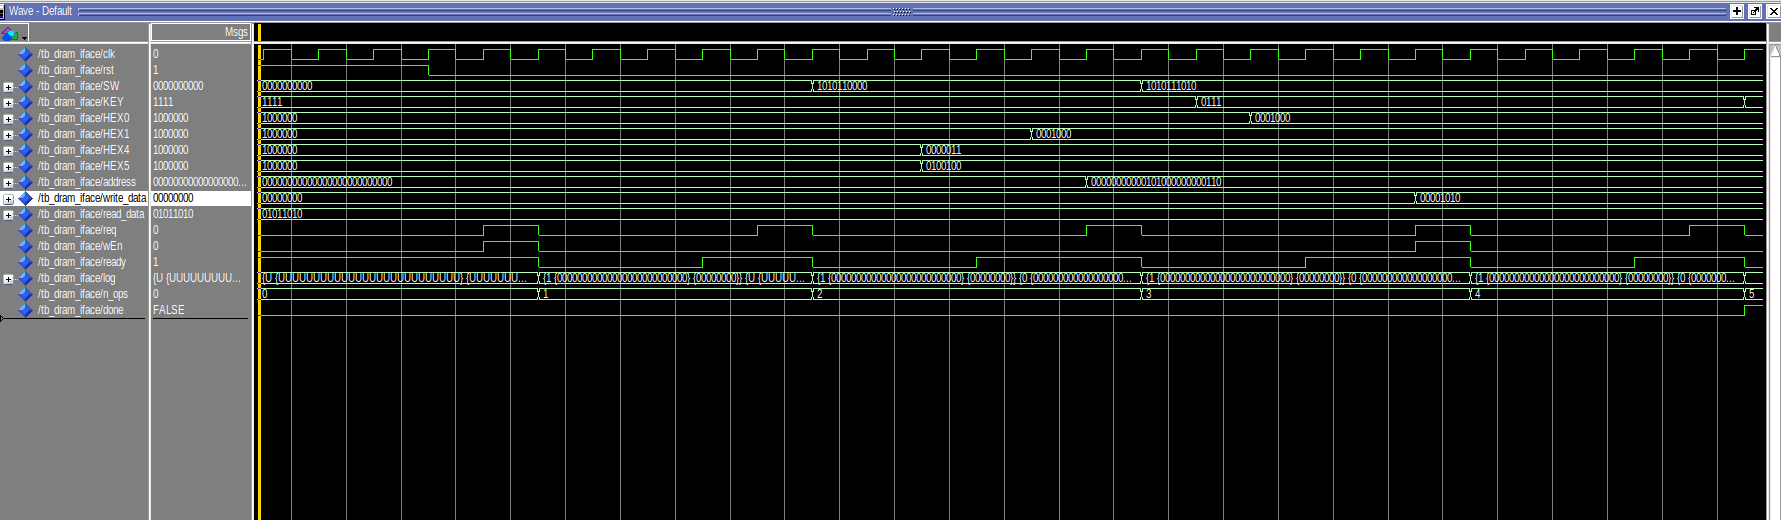
\includegraphics[width=\textwidth]{tb_iface.png}
  \caption{Simulação de \texttt{tb\_dram\_iface}: os cinco pulsos de \texttt{req}
  com os \texttt{wEn}/\texttt{address}/\texttt{write\_data} esperados.}
\end{figure}

\textbf{Por que isto prova a correção:} a forma de onda mostra exatamente os cinco
pulsos de \texttt{req} na ordem esperada, com \texttt{wEn=1} apenas nas escritas
(\texttt{op0}, \texttt{op3}) e o endereço/dado corretos em cada uma. Isso comprova
que a lógica de decisão da interface --- limpeza no reset, leitura ao trocar de
endereço, escrita por \texttt{KEY[3]} e read-back automático --- está correta,
independentemente do controlador real. Console: \texttt{tb\_dram\_iface: todos os
cenarios passaram}.

\subsection{Teste de componente: \texttt{tb\_dram\_controller.vhd}}
\textbf{Objetivo:} validar o protocolo SDRAM e, sobretudo, a temporização de
captura de leitura, sem a interface de usuário.

\textbf{Metodologia --- fidelidade ao hardware:} o testbench modela o SDRAM real
nos pinos \texttt{DRAM\_*} com \textbf{período de 7~ns ($\approx$143~MHz)},
\textbf{\texttt{DRAM\_CLK = not clk}}, \textbf{CAS latency 3} e \textbf{tAC =
5400~ps} (o dado de leitura só fica válido tAC após a borda do chip, modelado com
\texttt{DRAM\_DQ <= tb\_dq\_data after TAC}). Sem essa fidelidade o teste passaria
com um valor de captura errado, mascarando o bug que só aparece na placa. A espera
de inicialização é encurtada apenas na simulação via
\texttt{generic map (INIT\_WAIT\_CYCLES => 50)}, de modo que toda a atividade fica
visível desde o início (o teste todo cabe em cerca de 9\,$\mu$s). O testbench
decodifica os comandos (\texttt{dram\_cmd\_dec}), conta-os
(\texttt{n\_activate}, \texttt{n\_read}, \ldots) e tem guardas de contenção de
barramento e \emph{watchdog}.

\textbf{Cenários cobertos:}
\begin{itemize}
  \item INIT: inicialização completa (PRECHARGE, 8 AUTO REFRESH, LOAD MODE) e
        subida de \texttt{ready};
  \item WRITE \texttt{0x5A} no endereço A e READ de retorno (deve ler \texttt{0x5A});
  \item independência de endereços: WRITE \texttt{0x3C} em B, READ B
        (\texttt{0x3C}) e READ A novamente (ainda \texttt{0x5A});
  \item AUTO REFRESH espontâneo durante o período ocioso.
\end{itemize}
O procedimento \texttt{dram\_op} respeita a regra de handshake (esperar
\texttt{ready='0'} e depois \texttt{ready='1'}), evitando o erro de atraso por um.

\begin{figure}[H]
  \centering
  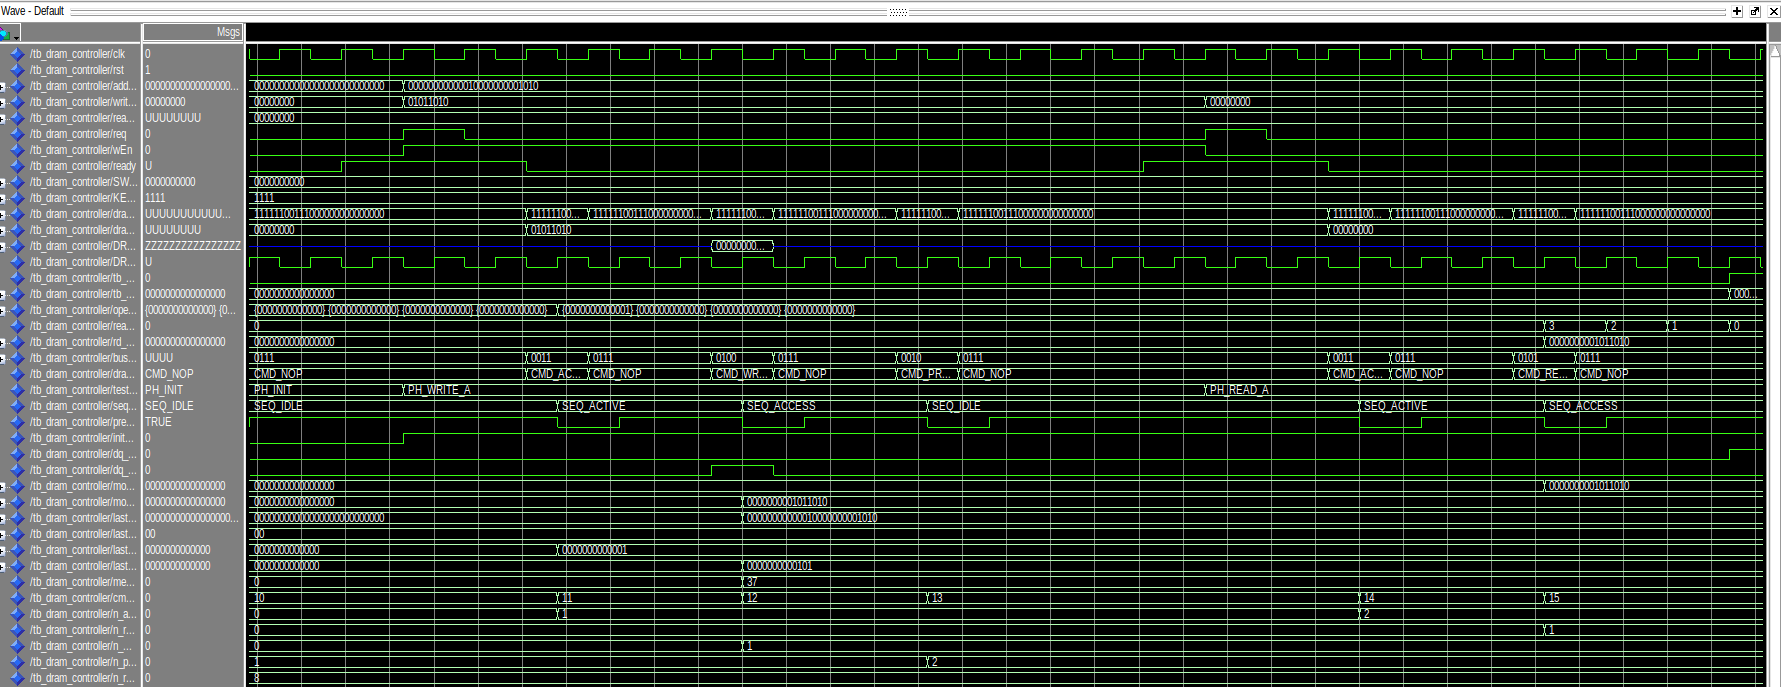
\includegraphics[width=\textwidth]{tb_controller.png}
  \caption{Simulação de \texttt{tb\_dram\_controller}: sequência
  ACTIVATE\,$\rightarrow$\,READ/WRITE\,$\rightarrow$\,PRECHARGE, o barramento
  \texttt{DRAM\_DQ} e a captura do dado dentro da janela válida.}
\end{figure}

\textbf{Por que isto prova a correção:} a forma de onda evidencia, para cada
operação, a sequência de comandos correta e o instante em que o dado válido aparece
em \texttt{DRAM\_DQ} (tAC após a borda do chip) sendo amostrado na borda de descida.
Os READs devolvem exatamente os valores escritos (\texttt{0x5A}/\texttt{0x3C}) e o
READ A repetido continua \texttt{0x5A}, provando armazenamento correto e
independência de endereços; o AUTO REFRESH aparece sozinho no ocioso. Console:
\texttt{tb\_dram\_controller: todos os cenarios passaram}.

\subsection{Teste de integração: \texttt{tb\_dram\_top\_level.vhd}}
\textbf{Objetivo:} validar o sistema completo (\texttt{iface
$\rightarrow$ reader $\rightarrow$ controller $\rightarrow$ SDRAM $\rightarrow$
display}) estimulando apenas \texttt{CLOCK\_50}, \texttt{SW} e \texttt{KEY}, como um
usuário na placa, e conferindo o valor mostrado em \texttt{HEX1}.

\textbf{Metodologia:} a PLL de simulação gera $\approx$143~MHz (não repassa os
50~MHz, para não mascarar a temporização de leitura) e levanta \texttt{locked} após
alguns ciclos. O testbench decodifica os comandos a partir dos pinos reais
\texttt{DRAM\_*\_N}, sincroniza as verificações com eventos observáveis
(\texttt{wait\_cmd} espera \texttt{CMD\_LOAD\_MODE}, \texttt{CMD\_WRITE},
\texttt{CMD\_READ}, \texttt{CMD\_AUTO\_REFRESH}) e compara \texttt{HEX1} com o padrão
de 7 segmentos esperado. A inicialização é encurtada via
\texttt{generic map (INIT\_WAIT\_CYCLES => 50)} para deixar a forma de onda legível
desde \texttt{t=0}. O testbench é compatível com VHDL-2002, rodando tanto no ghdl
quanto na RTL Simulation do Quartus (ModelSim-Altera).

\textbf{Cenários cobertos (a ``história''):}
\begin{itemize}
  \item RESET e INIT: solta o reset e espera o LOAD MODE REGISTER (init concluído),
        confirmando os 8 AUTO REFRESH;
  \item escreve 7 no endereço 1 via \texttt{KEY[3]} $\rightarrow$ \texttt{HEX1}
        mostra 7;
  \item seleciona o endereço 2 (nunca escrito) $\rightarrow$ \texttt{HEX1} mostra 0;
  \item volta ao endereço 1 $\rightarrow$ \texttt{HEX1} continua 7 (persistência);
  \item AUTO REFRESH espontâneo durante o ocioso.
\end{itemize}

\begin{figure}[H]
  \centering
  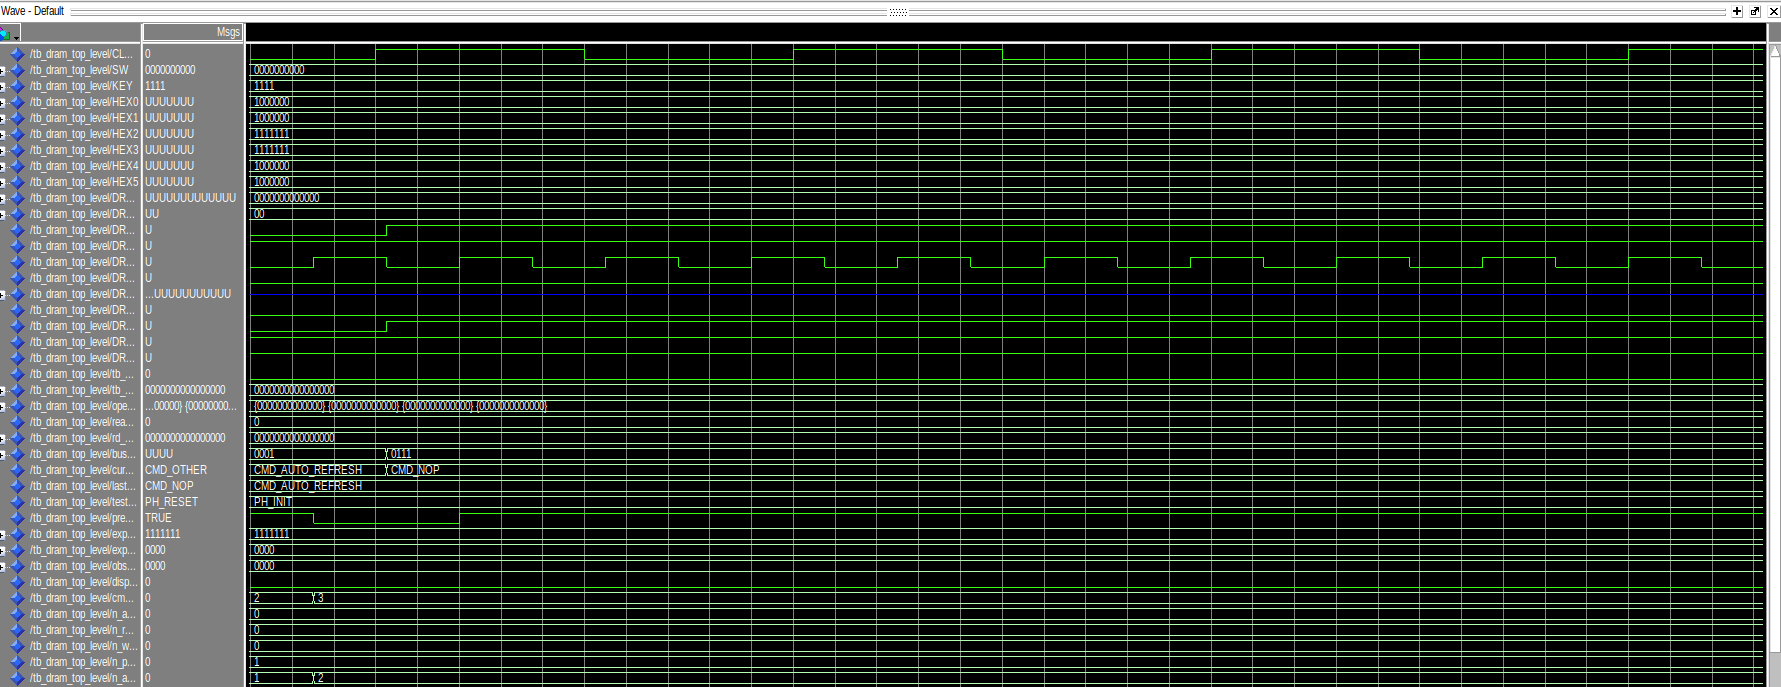
\includegraphics[width=\textwidth]{tb_toplevel.png}
  \caption{Simulação de \texttt{tb\_dram\_top\_level}: reset, init, escrita via
  \texttt{KEY[3]}, leituras e o valor final em \texttt{HEX1}.}
\end{figure}

\textbf{Por que isto prova a correção:} como nada interno é injetado, a forma de
onda demonstra o caminho completo funcionando: após o init, escrever 7 no endereço
1 faz \texttt{HEX1} exibir 7; mudar para um endereço virgem mostra 0; e
\textbf{voltar ao endereço 1 reexibe 7}, provando que o dado foi de fato gravado na
SDRAM e relido (persistência). O AUTO REFRESH espontâneo confirma a manutenção da
memória. Console: \texttt{tb\_dram\_top\_level: todos os cenarios passaram}.

\section{Análise de Execução}
\label{sec:analise}
\subsection{Captura do dado de leitura (o problema central)}
A maior dificuldade foi a leitura retornar \texttt{0xFF} em vez do dado gravado. A
causa era de temporização: a 143~MHz, o dado válido chega tAC após a borda do clock
do chip e essa janela cai \emph{entre} as bordas de subida do clock do sistema ---
amostrar na subida lia o barramento ainda em alta impedância. A solução foi
capturar \texttt{DRAM\_DQ} na \textbf{borda de descida} de \texttt{clk} (que, com
\texttt{DRAM\_CLK = not pll\_clk}, coincide com a subida do chip), usar
\texttt{READ\_CAPTURE\_CYCLES = 5} e o \emph{mode register} \texttt{0x230}
(CAS latency 3, burst length 1). Com CAS latency 2 (\texttt{0x220}) ou captura na
subida, o teste lê \texttt{0xFF} --- exatamente o sintoma original.

\subsection{Inicialização longa e parametrização por \emph{generic}}
A espera obrigatória de power-up do SDRAM dura 28600 ciclos (cerca de 200\,$\mu$s a
143~MHz), em que o barramento fica legitimamente em NOP. Em simulação isso deixava a
forma de onda ``parada'' (apenas os clocks oscilando) até 200\,$\mu$s. Expor essa
espera como o \emph{generic} \texttt{INIT\_WAIT\_CYCLES} (padrão 28600 na síntese,
sobrescrito para 50 nos testbenches) resolveu o problema sem alterar o
comportamento sintetizado: a atividade passou a ser visível desde \texttt{t=0}.

\subsection{Barramento \texttt{DRAM\_DQ} bidirecional}
O barramento de dados é bidirecional, com risco de contenção. A solução foi o
top-level dirigir \texttt{DRAM\_DQ} \emph{apenas} no ciclo do comando WRITE
(deixando-o em alta impedância no restante), enquanto o modelo de SDRAM nos
testbenches só dirige durante a leitura (após tAC). Os testbenches incluem guardas
concorrentes que falham se houver contenção (\texttt{X} no barramento ou dois
\emph{drivers} simultâneos).

\subsection{PLL: simulação versus síntese}
O ghdl não elabora a megafunção de PLL da Altera. Foi criado o
\texttt{pll\_sim\_stub.vhd}, que mantém a mesma entidade e gera um clock de
$\approx$143~MHz com \texttt{locked} atrasado --- garantindo que a simulação exerça
a mesma frequência e o mesmo caminho de reset por \texttt{locked} do hardware real.
Na síntese e na RTL Simulation do Quartus usa-se a PLL real; o stub é exclusivo da
simulação em ghdl.

\subsection{Sincronização de entradas e handshake}
\texttt{SW} e \texttt{KEY} são assíncronos: amostrá-los direto a 143~MHz pode levar
a FSM à metaestabilidade. A interface os sincroniza com dois flip-flops. No
handshake \texttt{req}/\texttt{ready}, foi essencial esperar \texttt{ready='0'}
(operação aceita) antes de \texttt{ready='1'} (operação concluída); checar apenas
\texttt{ready='1'} levaria a ler o dado da operação anterior (erro de atraso por um).

\end{document}
